\documentclass[11pt]{article}
\usepackage[margin=1in]{geometry}
\usepackage{amsmath, amssymb}
\usepackage{booktabs, tabularx}
\usepackage{enumitem}
\usepackage{xcolor}
\usepackage{tikz}
\usetikzlibrary{positioning, calc}
\usepackage{listings}

\definecolor{pygreen}{HTML}{2E8B57}
\definecolor{pyblue}{HTML}{2060A0}
\definecolor{pyred}{HTML}{C03030}
\definecolor{lightgray}{HTML}{F0F0F0}

\lstset{
  language=Python,
  basicstyle=\ttfamily,
  keywordstyle=\color{pyblue}\bfseries,
  stringstyle=\color{pygreen},
  commentstyle=\color{gray}\itshape,
  showstringspaces=false,
  frame=none,
  xleftmargin=0pt,
}

\newcommand{\py}[1]{\texttt{\color{pyblue}#1}}
\newcommand{\val}[1]{\ensuremath{V_{#1}}}

\begin{document}

\begin{center}
{\Large\bfseries Python Slice Notation: The Two-Choice Mental Model}\\[8pt]
{\itshape How colon placement and sign fully determine every one-sided slice}
\end{center}

\vspace{12pt}

%% ============================================================
\section{Setup: Index Map}
%% ============================================================

Given a list \py{a = [\val{0}, \val{1}, \val{2}, \val{3}, \val{4}]} of length 5:

\begin{center}
\renewcommand{\arraystretch}{1.3}
\begin{tabular}{r*{5}{c}}
\toprule
\textbf{Element}   & $\val{0}$ & $\val{1}$ & $\val{2}$ & $\val{3}$ & $\val{4}$ \\
\midrule
\textbf{Positive index} & \texttt{0} & \texttt{1} & \texttt{2} & \texttt{3} & \texttt{4} \\
\textbf{Negative index}  & \texttt{-5} & \texttt{-4} & \texttt{-3} & \texttt{-2} & \texttt{-1} \\
\bottomrule
\end{tabular}
\end{center}

\medskip
\noindent
Every position can be addressed by either its positive or negative index.
Positive indices count from the front ($0 \to n{-}1$); negative indices count from the back ($-1$ is the last element, $-n$ is the first).

%% ============================================================
\section{The Cut Metaphor}
%% ============================================================

Think of a slice index $n$ as placing a \textbf{cut} in the list---a vertical line between elements.
The cut falls \emph{before} the element at position $n$:

\begin{center}
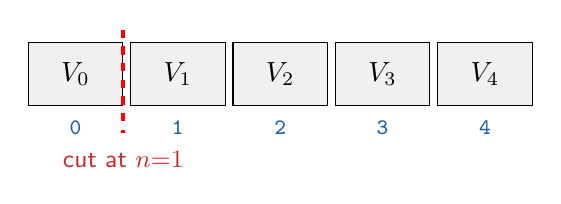
\begin{tikzpicture}[
    cell/.style={minimum width=1.2cm, minimum height=0.8cm, draw, fill=lightgray, font=\ttfamily},
    cutline/.style={ultra thick, red, dashed},
    label/.style={font=\small\sffamily, text=pyred},
  ]
  % cells
  \foreach \i/\v in {0/$\val{0}$, 1/$\val{1}$, 2/$\val{2}$, 3/$\val{3}$, 4/$\val{4}$} {
    \node[cell] (c\i) at (\i*1.3, 0) {\v};
  }
  % indices below
  \foreach \i in {0,...,4} {
    \node[below=2pt of c\i, font=\footnotesize\ttfamily, text=pyblue] {\i};
  }
  % cut before index 1
  \draw[cutline] ($(c0.north east)+(0,0.15)$) -- ($(c0.south east)+(0,-0.35)$);
  \node[label, below=0.45cm of c0.south east] {cut at $n{=}1$};
\end{tikzpicture}
\end{center}

\noindent
The slice then keeps everything on \emph{one side} of the cut.
Which side? That is determined by where the colon goes.

%% ============================================================
\section{The Four One-Sided Slices}
%% ============================================================

\begin{center}
\renewcommand{\arraystretch}{1.5}
\begin{tabular}{clccll}
\toprule
\textbf{Slice} & \textbf{Cut point} & \textbf{Keep side} & \textbf{Result} & \textbf{Mnemonic} \\
\midrule
\py{a[1:]}  & before index 1  & right $\rightarrow$ & \py{[\val{1}, \val{2}, \val{3}, \val{4}]} & ``drop the head''  \\
\py{a[:1]}  & before index 1  & left $\leftarrow$  & \py{[\val{0}]}                             & ``only the head''  \\
\py{a[-1:]} & before index $-1$ & right $\rightarrow$ & \py{[\val{4}]}                             & ``only the tail''  \\
\py{a[:-1]} & before index $-1$ & left $\leftarrow$  & \py{[\val{0}, \val{1}, \val{2}, \val{3}]} & ``drop the tail''  \\
\bottomrule
\end{tabular}
\end{center}

%% ============================================================
\section{The Two-Choice Rule}
%% ============================================================

Every one-sided slice is determined by exactly \textbf{two binary choices}:

\begin{enumerate}[label=\textbf{\arabic*.}, leftmargin=2em, itemsep=6pt]
  \item \textbf{Sign of $n$} --- \emph{where} to cut.
    \begin{itemize}[nosep]
      \item Positive $n$ $\;\Rightarrow\;$ count from the \textbf{front} (left).
      \item Negative $n$ $\;\Rightarrow\;$ count from the \textbf{back} (right).
    \end{itemize}

  \item \textbf{Colon placement} --- \emph{which side} to keep.
    \begin{itemize}[nosep]
      \item \py{n:} (colon \emph{after}) $\;\Rightarrow\;$ keep everything \textbf{after} the cut (right side).
      \item \py{:n} (colon \emph{before}) $\;\Rightarrow\;$ keep everything \textbf{before} the cut (left side).
    \end{itemize}
\end{enumerate}

\begin{center}
\fbox{\parbox{0.85\textwidth}{\centering
\textbf{Colon placement = which side you keep.\quad Sign = where you cut.}
}}
\end{center}

%% ============================================================
\section{Visual Summary}
%% ============================================================

\begin{center}
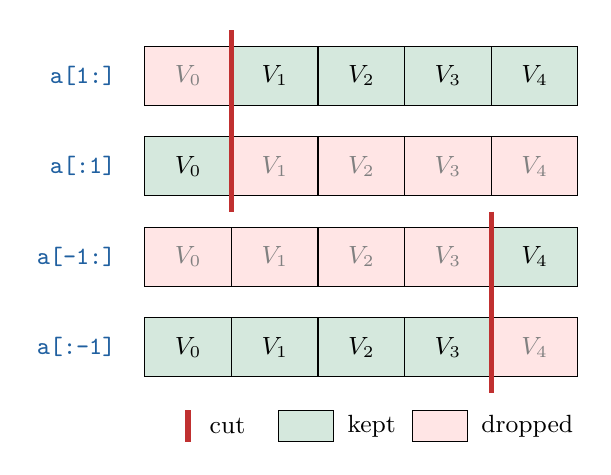
\begin{tikzpicture}[
    cell/.style={minimum width=1.1cm, minimum height=0.75cm, draw, font=\ttfamily\small,
                 outer sep=0pt, inner sep=0pt},
    kept/.style={cell, fill=pygreen!20},
    dropped/.style={cell, fill=red!10, text=gray},
    cutline/.style={line width=2pt, pyred},
    slabel/.style={font=\ttfamily\small\bfseries, text=pyblue, anchor=east},
  ]

  \def\cellw{1.1}   % cell pitch = cell width (no gaps)
  \def\rowh{1.15}    % vertical pitch between rows

  % --- a[1:] ---
  \def\ry{0}
  \node[slabel] at (-0.8, \ry) {a[1:]};
  \node[dropped] (a0) at (0,\ry) {$\val{0}$};
  \node[kept]    (a1) at (\cellw,\ry) {$\val{1}$};
  \node[kept]    (a2) at (2*\cellw,\ry) {$\val{2}$};
  \node[kept]    (a3) at (3*\cellw,\ry) {$\val{3}$};
  \node[kept]    (a4) at (4*\cellw,\ry) {$\val{4}$};
  \draw[cutline] ($(a0.north east)+(0,0.2)$) -- ($(a0.south east)-(0,0.2)$);

  % --- a[:1] ---
  \def\ry{-\rowh}
  \node[slabel] at (-0.8, \ry) {a[:1]};
  \node[kept]    (b0) at (0,\ry) {$\val{0}$};
  \node[dropped] (b1) at (\cellw,\ry) {$\val{1}$};
  \node[dropped] (b2) at (2*\cellw,\ry) {$\val{2}$};
  \node[dropped] (b3) at (3*\cellw,\ry) {$\val{3}$};
  \node[dropped] (b4) at (4*\cellw,\ry) {$\val{4}$};
  \draw[cutline] ($(b0.north east)+(0,0.2)$) -- ($(b0.south east)-(0,0.2)$);

  % --- a[-1:] ---
  \def\ry{-2*\rowh}
  \node[slabel] at (-0.8, \ry) {a[-1:]};
  \node[dropped] (c0) at (0,\ry) {$\val{0}$};
  \node[dropped] (c1) at (\cellw,\ry) {$\val{1}$};
  \node[dropped] (c2) at (2*\cellw,\ry) {$\val{2}$};
  \node[dropped] (c3) at (3*\cellw,\ry) {$\val{3}$};
  \node[kept]    (c4) at (4*\cellw,\ry) {$\val{4}$};
  \draw[cutline] ($(c3.north east)+(0,0.2)$) -- ($(c3.south east)-(0,0.2)$);

  % --- a[:-1] ---
  \def\ry{-3*\rowh}
  \node[slabel] at (-0.8, \ry) {a[:-1]};
  \node[kept]    (d0) at (0,\ry) {$\val{0}$};
  \node[kept]    (d1) at (\cellw,\ry) {$\val{1}$};
  \node[kept]    (d2) at (2*\cellw,\ry) {$\val{2}$};
  \node[kept]    (d3) at (3*\cellw,\ry) {$\val{3}$};
  \node[dropped] (d4) at (4*\cellw,\ry) {$\val{4}$};
  \draw[cutline] ($(d3.north east)+(0,0.2)$) -- ($(d3.south east)-(0,0.2)$);

  % --- Legend ---
  \def\ly{-3*\rowh - 1.0}
  \draw[cutline] (0, \ly-0.2) -- (0, \ly+0.2);
  \node[font=\small, right] at (0.15, \ly) {cut};
  \node[kept, minimum width=0.7cm, minimum height=0.4cm] at (1.5, \ly) {};
  \node[font=\small, right] at (1.9, \ly) {kept};
  \node[dropped, minimum width=0.7cm, minimum height=0.4cm] at (3.2, \ly) {};
  \node[font=\small, right] at (3.6, \ly) {dropped};

\end{tikzpicture}
\end{center}

%% ============================================================
\section{Common Idioms}
%% ============================================================

\begin{center}
\renewcommand{\arraystretch}{1.4}
\begin{tabular}{lll}
\toprule
\textbf{Pattern} & \textbf{Meaning} & \textbf{Example (len 5)} \\
\midrule
\py{a[k:]}   & skip the first $k$ elements            & \py{a[2:]} $\to$ \py{[\val{2}, \val{3}, \val{4}]} \\
\py{a[:k]}   & take the first $k$ elements             & \py{a[:2]} $\to$ \py{[\val{0}, \val{1}]} \\
\py{a[-k:]}  & take the last $k$ elements              & \py{a[-2:]} $\to$ \py{[\val{3}, \val{4}]} \\
\py{a[:-k]}  & drop the last $k$ elements              & \py{a[:-2]} $\to$ \py{[\val{0}, \val{1}, \val{2}]} \\
\midrule
\py{a[:]}    & shallow copy (keep everything)          & \py{[\val{0}, \val{1}, \val{2}, \val{3}, \val{4}]} \\
\py{a[:0]}   & empty (cut before front, keep left of that) & \py{[]} \\
\py{a[0:]}   & everything (cut before front, keep right)    & same as \py{a[:]} \\
\bottomrule
\end{tabular}
\end{center}

%% ============================================================
\section{Key Insight: Symmetry of Complements}
%% ============================================================

For any index $n$, the slices \py{a[:n]} and \py{a[n:]} are \textbf{complementary}---they partition the list with no overlap and no gap:

\[
\texttt{a[:n]} \;+\; \texttt{a[n:]} \;=\; \texttt{a}
\qquad \text{for all valid } n
\]

This means:
\begin{itemize}[nosep]
  \item \py{a[:1]} $+$ \py{a[1:]} $=$ \py{a} \quad (head + rest = whole)
  \item \py{a[:-1]} $+$ \py{a[-1:]} $=$ \py{a} \quad (body + tail = whole)
\end{itemize}

\noindent
If you remember what one slice does, you automatically know what its mirror does---it's the complementary partition.

\end{document}
